\documentclass[10pt,handout]{beamer}
\usepackage{amsmath}
\usepackage[bb=dsserif]{mathalpha}
\usepackage{bm}
\usetheme{CambridgeUS}
%%%%%%%%%%%%%%%%%%%%%%%%%%%%%%
% 3.2. フォントの設定
%%%%%%%%%%%%%%%%%%%%%%%%%%%%%%
%\renewcommand{\kanjifamilydefault}{\gtdefault} % 和文既定をゴシックに変更
\usefonttheme{structurebold} %Beamerによるフォントの置き換えを阻止
% コマンドの説明は註18を参照
%\usepackage[deluxe]{otf}
%\usepackage[noalphabet]{pxchfon}
%\setboldgothicfont{HaranoAjiGothic-Medium.otf} %\bfseriesの設定
%%%%%%%%%%%%%%%%%%%%%%%%%%%%%%
% 3.4. テーマの配色をいじる
%%%%%%%%%%%%%%%%%%%%%%%%%%%%%%
\usecolortheme{default}
\setbeamercolor{structure}{fg=red}
%%%%%%%%%%%%%%%%%%%%%%%%%%%%%%
% 3.5. フレーム番号の調整
%%%%%%%%%%%%%%%%%%%%%%%%%%%%%%
\setbeamertemplate{footline}[frame number]
\setbeamerfont{page number in head/foot}{size=\normalsize}
\setbeamercolor{page number in head/foot}{fg=gray}
%%%%%%%%%%%%%%%%%%%%%%%%%%%%%%
% 3.6. フレームタイトルの強調
%%%%%%%%%%%%%%%%%%%%%%%%%%%%%%
\setbeamerfont{frametitle}{series=\bfseries}
%%%%%%%%%%%%%%%%%%%%%%%%%%%%%%
% 3.7. 脚註番号を設定
%%%%%%%%%%%%%%%%%%%%%%%%%%%%%%
\renewcommand{\thefootnote}{\textasteriskcentered\arabic{footnote}}
%%%%%%%%%%%%%%%%%%%%%%%%%%%%%%
% 3.8. 余白を広げる
%%%%%%%%%%%%%%%%%%%%%%%%%%%%%%
\setbeamersize{text margin left=15pt, text margin right=25pt}
\newcommand{\textred}[1]{\textcolor{red}{#1}}

%------------------------------------------------------------
%This block of code defines the information to appear in the
%Title page
\title[Weekly Presentation] %optional
{Weekly Presentation: \\
Political Life Cycles \\
J. Melnick, A. Smith, and B. Mesquita (2024)}

% \subtitle{A short story}

\author[Hiromu Sugiyama] % (optional)
{Hiromu Sugiyama}

\date[April 8th, 2025] % (optional)
{New Direction to Formal Theory, Spring 2025}


%End of title page configuration block
%------------------------------------------------------------



%------------------------------------------------------------
%The next block of commands puts the table of contents at the 
%beginning of each section and highlights the current section:

\AtBeginSection[]
{
  \begin{frame}
    \frametitle{Table of Contents}
    \tableofcontents[currentsection]
  \end{frame}
}
%------------------------------------------------------------


\begin{document}

%The next statement creates the title page.
\frame{\titlepage}


%---------------------------------------------------------
%This block of code is for the table of contents after
%the title page
\begin{frame}
\frametitle{Table of Contents}
\tableofcontents
\end{frame}
%---------------------------------------------------------

\section{Motivation}
%---------------------------------------------------------
%Changing visivility of the text
\begin{frame}
\frametitle{Motivation}
\begin{itemize}
    \item Motivation: the observed pattern that leaders often become less transparent, more corrupt, and more repressive over time
    \item Building on selectorate theory, this paper develops and tests a theory of political life cycle effects, explaining how a leader’s survival-motivated allocation of public and private goods shifts over time during tenure
\end{itemize}
\end{frame}
%---------------------------------------------------------

\section{Selectorate Theory Basics}
%---------------------------------------------------------
%Changing visivility of the text
\begin{frame}
\frametitle{Selectorate Theory Basics (BDM et al., 2003)}
\begin{itemize}
    \item[] Players: 
    \begin{itemize}
        \item Leader(s)
        \item Challenger(s)
        \item People in society
        \begin{itemize}
            \item[-] Selectorate: Subset of people with at least nominal say in choosing the leader
            \item[-] Winning Coalitions: Subset of selectorate that endows the leader with the sufficient power over the remainder of selectorate and people in society not included in electorate 
        \end{itemize}
    \end{itemize}
    \item[] Two key variables:
    \begin{itemize}
        \item W = Size of winning coalition
        \item S = Size of selectorate 
    \end{itemize}
\end{itemize}
\end{frame}
%---------------------------------------------------------

%---------------------------------------------------------
%Changing visivility of the text
\begin{frame}
\frametitle{Selectorate Theory Basics (BDM et al., 2003)}
\begin{itemize}
    \item[] Leaders' Actions: 
    \begin{itemize}
        \item Provide public goods to all the selectorate and private goods only to the members of winning coalition
        \item Maintain the coalition size to the winning coalition size W, to remain in power
        \item Offer at least as many private goods as the challengers to the overlapping members within both coalitions
    \end{itemize}
    \item[] Challengers' Actions:
    \begin{itemize}
        \item Similarly, maintain the coalition size to the winning coalition size W
        \item Take at least one of the leaders' coalition member by offer at least as many private goods as the leader do to the overlapping members within both coalitions
    \end{itemize} 
\end{itemize}
\end{frame}
%---------------------------------------------------------

%---------------------------------------------------------
%Changing visivility of the text
\begin{frame}
\frametitle{Selectorate Theory Basics (BDM et al., 2003)}
\begin{itemize}
    \item[] \textbf{Affinity}: likes and trusts towards some selectorates 
    \begin{itemize}
        \item In the equilibrium, the theory predicts the leader to win because of the uncertainty of challenger's affinity
        \item Here, leader is advantageous because, upon coming to the power, the affinities are revealed whereas a selectorate is in the challenger's affinity with the probability $\frac{W}{S}$
    \end{itemize}
\end{itemize}
\end{frame}
%---------------------------------------------------------

\section{Political Life Cycle Model}
%---------------------------------------------------------
%Changing visivility of the text
\begin{frame}
\frametitle{Key Innovation -- Gradual Learning}
\begin{itemize}
    \item Instead of leader's affinity revealed immediately, the new model takes revelation of affinities as a \textbf{gradual learning process}
    \item As leaders retains longer, she learns more and more about her own affinity for her coaltion.
    \item Selectorates, in turn, are initially uncertain, he can be fairly certain if he is not replaced from the coalition for many periods. 
\end{itemize}
\end{frame}
%---------------------------------------------------------

%---------------------------------------------------------
%Changing visivility of the text
\begin{frame}
\frametitle{Model Setup (3.1 pg.7)}
\begin{itemize}
    \item Players:
    \begin{itemize}
        \item Leader \textit{L}
        \item Coalition members \textit{W}
        \item Mass public \textit{M}
    \end{itemize}
    \item Consider an indefinite repeated game $(t = 0, 1, 2, ...)$ where
    \begin{itemize}
        \item[1.] \textit{L} forms a coalition of size \textit{W} and offer them with public ($g_t$) and private ($z_t$) goods
        \item[2.] \textit{M} decide to rebel or not
        \item[3.] \textit{W} decide whether to depose, and if \textit{M} rebels, whether to suppress the masses or tacitly allow revolution to succeed
    \end{itemize}
\end{itemize}
\end{frame}
%---------------------------------------------------------

%---------------------------------------------------------
%Changing visivility of the text
\begin{frame}
\frametitle{Model Setup: Loyalty and Willingness to Suppress (3.1 pg.7)}
\begin{itemize}
    \item In step 3 of repeated game, loyalty of \textit{W} (deposition) and their willingness to suppress depends on:
    \begin{itemize}
        \item[1.] Immediate policy rewards: public/private goods ($g_t, z_t$)
        \item[2.] Leader's performances: valence shock ($\theta_t$)
        \item[3.] Expectation of members being retained and rewarded in future coalition: critical to coalition dynamics as leader learns her affinity
    \end{itemize}
\end{itemize}
\end{frame}
%---------------------------------------------------------

%Changing visivility of the text
\begin{frame}
\frametitle{Model Setup: Learning Dynamics (3.1 pg.8)}
\begin{itemize}
    \item Every potential coalition member has affinity types: $\alpha_H, \alpha_L$
    \item Let $\alpha_0$, proportion of high type at $t = 0$ ($W < \alpha_0$)
    \item Note that leader is \textbf{uncertain} about her affinity and the members has incentive for opacity:
    \begin{itemize}
        \item Leader reassures members; risky to tipping off their replacement
        \item Members have incentives to act and say in favor of leader
    \end{itemize}
    \item[] $\Rightarrow$ leader cannot immediately recognize $\alpha_L$, and gradually learns who is who
\end{itemize}
\end{frame}
%---------------------------------------------------------

%Changing visivility of the text
\begin{frame}
\frametitle{Model Setup: Learning Dynamics (3.1 pg.8)}
\begin{itemize}
    \item At the end of each period, leader assumes to detect a low affinity type with probability \textit{q}, replace them
    \item Here, denote $\alpha_t$ as proportion of high affinity type in the leader's coalition at the start of period t and $\alpha_{t+1}$ as the proportion at the end (or start of next period)
    \item The model assumes that the coalition is made up of continuum of members rather than discrete individuals
\end{itemize}
\end{frame}
%---------------------------------------------------------

%---------------------------------------------------------
%Changing visivility of the text
\begin{frame}
\frametitle{Stage Game: Steps (3.2 pg.9)}
\begin{itemize}
    \item[] The game starts when a new leader comes to power with an initial coalition members of size \textit{W}. Within each period \textit{t}, the following happens:
    \begin{itemize}
        \item[1.] Policy formation: Leader offers public ($g_t$) and private goods ($z_t$)
        \item[2.] Revolution Choice: Masses observes the cost of rebel ($K_t$) and decide to rebel
        \begin{itemize}
            \item $K_t \sim$ H(x) = Pr($K_t \leq$ x)
            \item Use uniform distribution for simplicity
        \end{itemize}
        \item[3.] Deposition and suppression choice: Coalition member observes a valence shock ($\theta_t$) and decide the next action accordingly (i.e. retain/depose/suppress/acquiesce)
        \begin{itemize}
            \item $\theta_t \sim$ i.i.d F(x) = Pr($\theta_t \leq x$)
            \item Assume: F($\cdot$) is strictly concave, continuous and twice differentiable and focus on exponential distribution.
        \end{itemize}
        \item[4.] Learning: Leader identifies low-affinity type by probability q if retain her power, and replaced with alternative selectorate
    \end{itemize}
\end{itemize}
\end{frame}
%---------------------------------------------------------
%---------------------------------------------------------
%Changing visivility of the text
\begin{frame}
\frametitle{Stage Game: Figure (pg.12)}
\begin{figure}
    \centering
    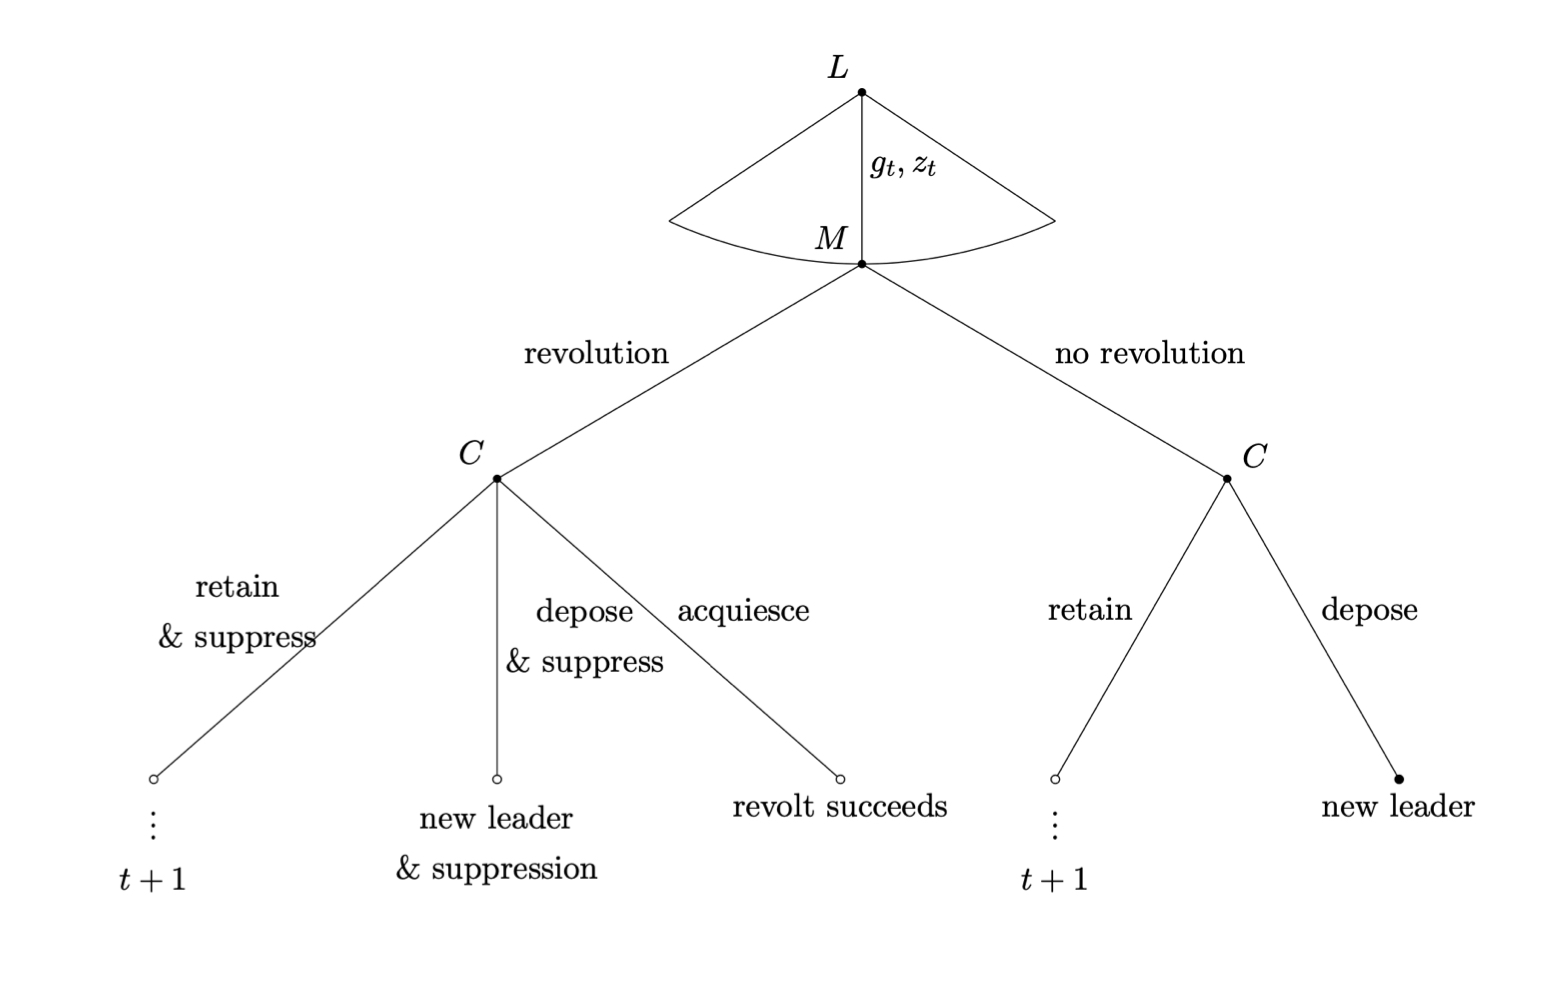
\includegraphics[width=0.93\linewidth]{Figure_1.jpeg}
    \caption{The Game Tree}
    \label{fig:enter-label}
\end{figure}
\end{frame}
%---------------------------------------------------------

%---------------------------------------------------------
%Changing visivility of the text
\begin{frame}
\frametitle{Payoff: Coalition/Mass Utility (pg.10)}
\begin{itemize}
    \item[] \textbf{Coalition members:}
    \begin{align*}
        U_W = 
        \begin{cases}
            u(g_t, z_t) - \theta_t + y_t &\text{if no revolution and leader retains} \\
            c_W &\text{if no revolution and leader deposed} \\
            r_W &\text{if revolution and succeeds} \\
            \gamma &\text{only when shuffled out}
        \end{cases}
    \end{align*}
    where
    \begin{itemize}
        \item[-] $y_t$: the net present value of future rewards
        \item[-] $u(\cdot, \cdot)$: additively separable, concave, and twice differentiable
        \item[-] $\gamma < c_W$: Assumption that reshuffled out is worse off than remaining in the coalition 
    \end{itemize}
\end{itemize}
\end{frame}
%---------------------------------------------------------

%---------------------------------------------------------
%Changing visivility of the text
\begin{frame}
\frametitle{Payoff: Coalition/Mass Utility (pg.10)}
\begin{itemize}
    \item[] \textbf{Coalition members (cont.):}
    \begin{align*}
        U_W = 
        \begin{cases}
            u(g_t, z_t) - \theta_t + y_t - \eta &\text{if revolution, retain \& suppress} \\
            c_W - \frac{\eta}{2} &\text{if revolution, deposed \& suppress}
        \end{cases}
    \end{align*}
    where
    \begin{itemize}
        \item $\eta, \frac{\eta}{2}$: the cost of suppressing the mass
        \item cost when leader retain $>$ cost when leader is deposed: the impetus of revolution weakens without leader whom the people are rebelling
    \end{itemize}
\end{itemize}
\end{frame}
%---------------------------------------------------------

%---------------------------------------------------------
%Changing visivility of the text
\begin{frame}
\frametitle{Payoff: Coalition/Mass Utility (pg.10)}
\begin{itemize}
    \item[] \textbf{Mass:}
    \begin{align*}
        U_M = 
        \begin{cases}
            u(g_t, 0) - \theta_t + y_t &\text{if no revolution and leader retains} \\
            c_M &\text{if no revolution and leader deposed} \\
            u(g_t, 0) - K_t &\text{if revolution, retain \& suppress} \\
            c_M - K_t &\text{if revolution, deposed \& suppress} \\
            r_M - K_t &\text{if revolution and succeeds}
        \end{cases}
    \end{align*}
    where
    \begin{itemize}
        \item $K_t$: cost of rebellion
    \end{itemize}
\end{itemize}
\end{frame}
%---------------------------------------------------------


%---------------------------------------------------------
%Changing visivility of the text
\begin{frame}
\frametitle{Payoff: Table (pg.11)}
\begin{figure}
    \centering
    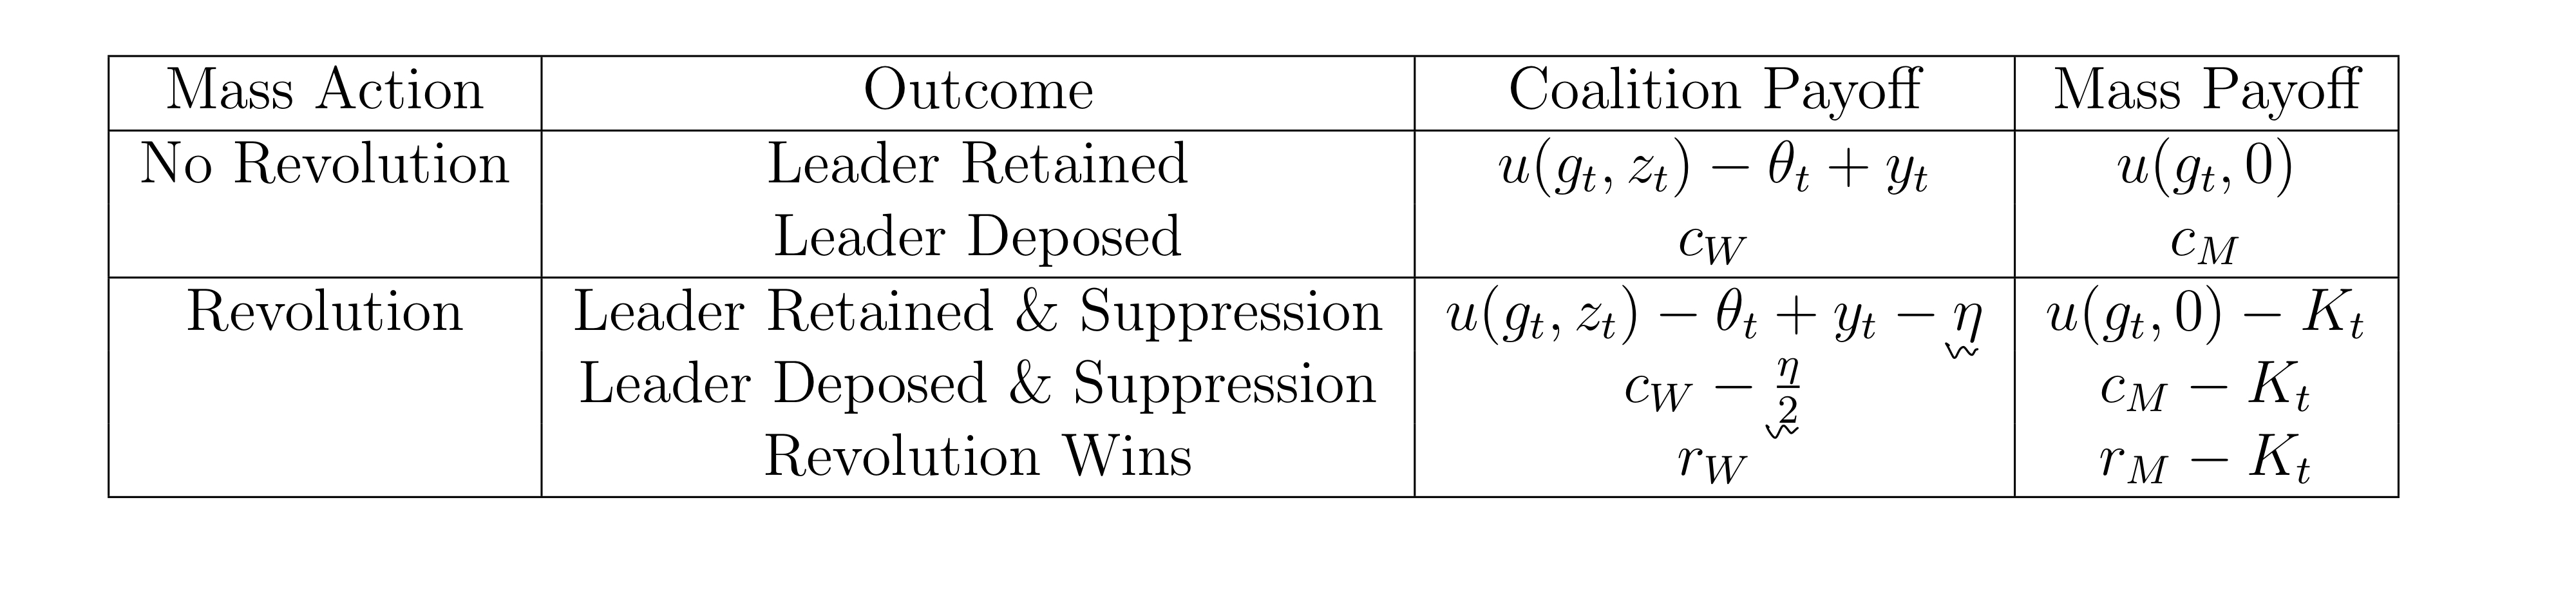
\includegraphics[width=1.1\linewidth]{Table1.jpeg}
    \caption{Payoff Table}
    \label{fig:enter-label}
\end{figure}
\end{frame}
%---------------------------------------------------------

%---------------------------------------------------------
%Changing visivility of the text
\begin{frame}
\frametitle{Payoff: Incumbent Utility (pg.11)}
\begin{itemize}
    \item Leader has a payoff:
    \[
        U_L(g_t, z_t) = \mathbb{1}_{\text{survive}}\Psi + R - pg_t - Wz_t + \mu\alpha_{t+1}
    \]
    \item Incumbent leader's utility depends on three components
    \begin{itemize}
        \item[-] Survival in office: $\Psi$ (office holding benefit)
        \item[-] Resource retention: $R - pg_t - W z_t$
        \item[-] Surrounded by high affinity type: $\mu \alpha_{t+1}$, which $\mu$ refers to the weight the leader places on future coalition loyalty
    \end{itemize}
    \item Leaders operate under budget constraints: $p g_t + Wz_t \leq R$
    \item[] where 
    \begin{itemize}
        \item[-] $R$: revenue 
        \item[-] $p$: cost of public good 
        \item[-] $W$: the effective cost of private good (i.e. coalition size)
    \end{itemize}
\end{itemize}
\end{frame}
%---------------------------------------------------------

\section{Theoretical Analysis}
%---------------------------------------------------------
%Changing visivility of the text
\begin{frame}
\frametitle{Analysis: Overview}
\begin{itemize}
    \item With the game and the payoffs, the paper characterizes the unique subgame perfect equilibrium in weakly undominated strategies.
    \item Few additional notes:
    \begin{itemize}
        \item $\delta$: common discount factor among coalition members
        \item Assume leader and mass maximize payoffs on a period-by-period basis
    \end{itemize}
\end{itemize}
\end{frame}
%---------------------------------------------------------

%---------------------------------------------------------
%Changing visivility of the text
\begin{frame}
\frametitle{Analysis: Learning Technology (pg.12-13)}
\begin{itemize}
    \item By Bayes Rule, the share of high affinity type in the coalition at the start of period $t$ is:
    \begin{align*}
        \alpha_t &= \frac{\alpha_0}{\alpha_0 + (1-\alpha_0)\text{Pr(not identified before period t)}} \\
        &= \frac{\alpha_0}{\alpha_0 + (1-\alpha_0)(1 - q)^t}
    \end{align*}
    \item[] where
    \begin{itemize}
        \item[-] $\alpha_0 = Pr(\alpha_H)$: initial proportion of people that leader has high affinity for the member
        \item[-] $Pr(\text{identify}|\alpha_L) = q$: probability the leader identifies the low affinity member; assume no false positive
    \end{itemize}
\end{itemize}
\end{frame}
%---------------------------------------------------------

%---------------------------------------------------------
%Changing visivility of the text
\begin{frame}
\frametitle{Analysis: Learning Technology (pg. 12-13)}
\begin{itemize}
    \item $\rho_t$: likelihood the member is removed from the coalition in period $t$
    \item[] $\rightarrow$ Overtime, the rate of leader replacing the member declines (learning makes better distinguishable)
    \item[] $\rightarrow$ The longer a member stays, the greater their expectation that the leader keep them in her coalition in the future
    \item Formally:
    \[
        \rho_t = (1-\alpha_t)q = \frac{q(1-\alpha_0)(1-q)^t}{\alpha_0 + (1-\alpha_0)(1-q)^t}
    \]
    \item[] where
    \begin{itemize}
        \item[-] $Pr(1-\alpha_t)$: share of low affinity type at time $t$
        \item[-] $Pr(\text{identify}|\alpha_L) = q$: probability the leader identifies the low affinity member; assume no false positive
    \end{itemize}
\end{itemize}
\end{frame}
%---------------------------------------------------------

%---------------------------------------------------------
%Changing visivility of the text
\begin{frame}
\frametitle{Analysis: Preposition 1 (pg. 12-13)}
\vfill
\begin{block}{Preposition 1}
    The probability of being reshuffled from the coalition declines over time. In the limit, as $t \xrightarrow[]{} \infty$, $\rho_t \xrightarrow[]{} 0$ and $\alpha_t \xrightarrow[]{} 1$
\end{block}
\begin{figure}
    \centering
    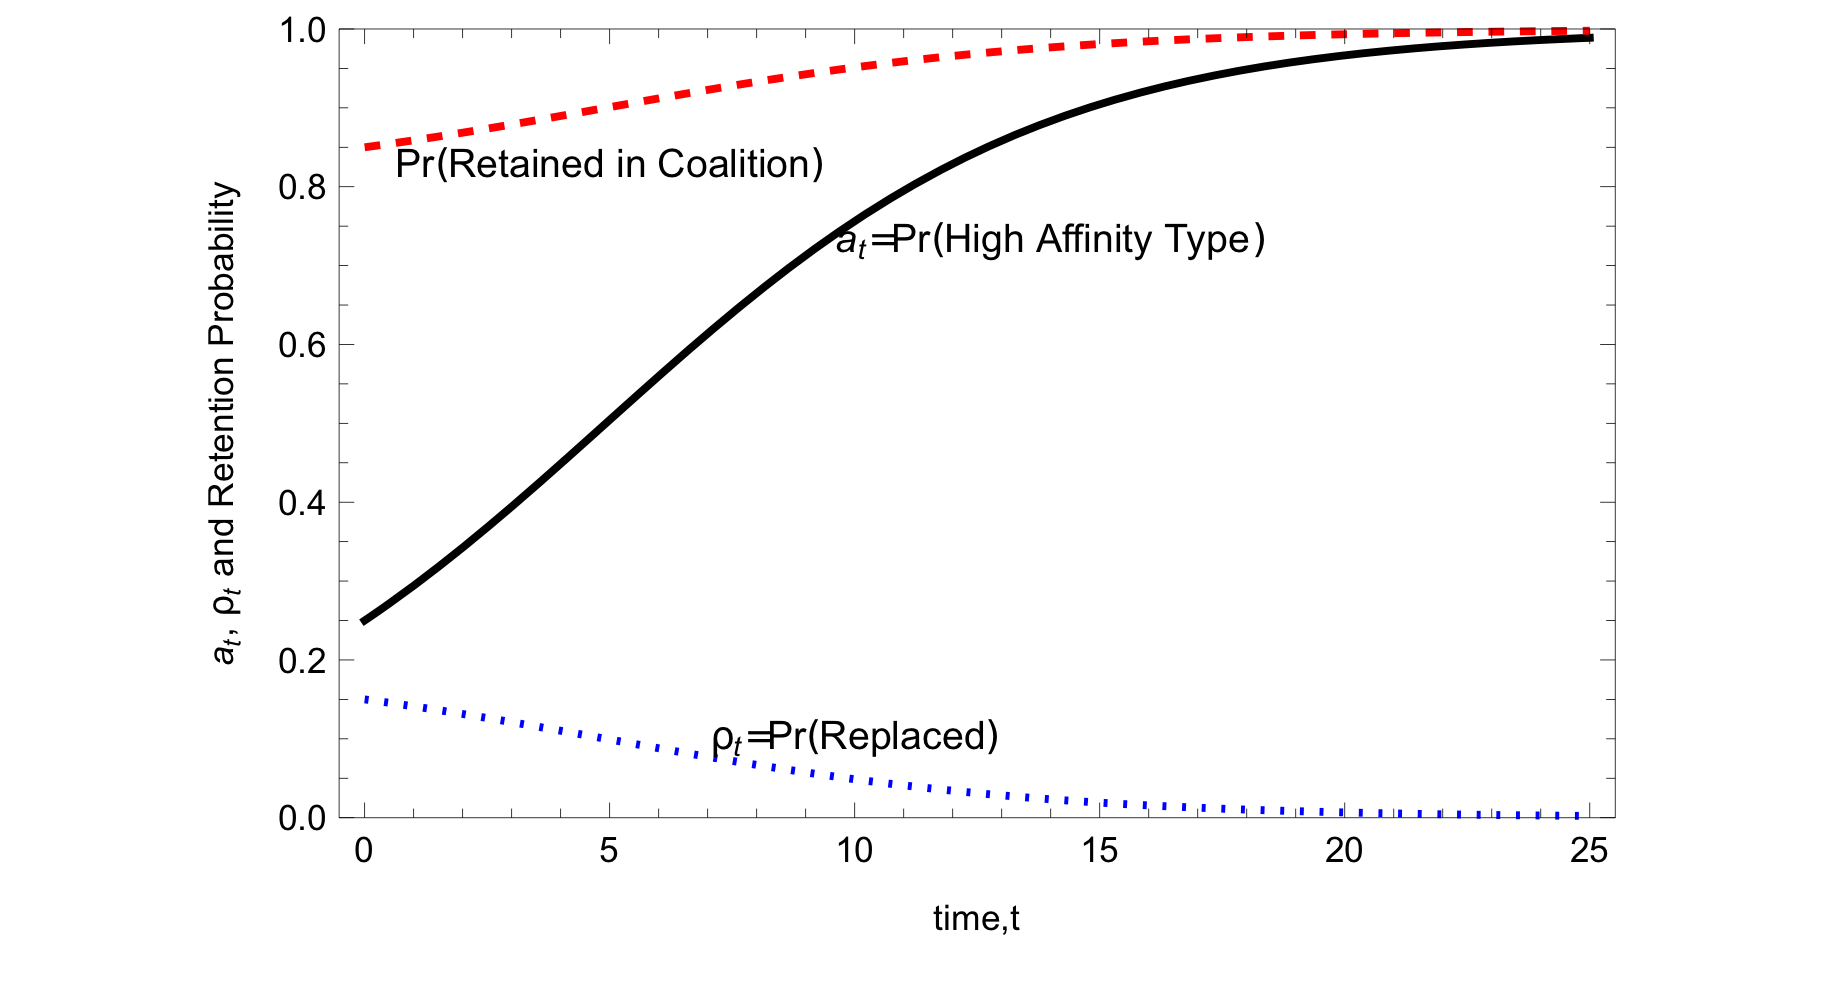
\includegraphics[width=0.75\linewidth]{Figure2.jpeg}
    \caption{Learning Dynamics and Coalition Reshuffles}
    \label{fig:enter-label}
\end{figure}
\end{frame}
%---------------------------------------------------------

%---------------------------------------------------------
%Changing visivility of the text
\begin{frame}
\frametitle{Analysis: Net Present Value (pg. 14)}
\begin{itemize}
    \item $Y_t$: expected value of being in the coalition at the start of period $t$
    \item $y_t$: continuation value of coalition member after political deposition stage (i.e. after step 3, before step 4)
    \begin{itemize}
        \item incumbent holds the member in her coalition
        \item incumbent replaces the member from the coalition
    \end{itemize}
    \item Formally,
    \[
        y_t = \delta(1-\rho_t)Y_{t+1} + \delta\rho_t\gamma
    \]
    \item With this value in mind, the paper derives the occurrence of revolutions, the coalition's choice, and the optimal policy allocations by leader.
\end{itemize}
\end{frame}
%---------------------------------------------------------

%---------------------------------------------------------
%Changing visivility of the text
\begin{frame}
\frametitle{Analysis: Suppression, Deposition, and Revolution (pg. 15)}
\begin{itemize}
    \item Suppose the leader offers public ($g_t$) and private ($z_t$) goods, then the policies worth $u(g_t, z_t)$ to coalition members and $u(g_t, 0)$ to the mass
    \item If no revolution, member chose either to retain or depose the leader
    \item Members prefer to retain their leader if
    \[
        \theta_t \leq \hat{\theta_t} = u(g_t, z_t) + y_t - c_W
    \]
    $\rightarrow$ Leader retains if the current dissatisfaction with her performance (i.e. $\theta_t$) is smaller than the dissatisfaction she is expected to produce for the members compared to their value if she is deposed. \par
    $\rightarrow$ Modified utility comparison (i.e. $u(g_t, z_t) - \theta_t + y_t \geq c_W$)    
\end{itemize}
\end{frame}
%---------------------------------------------------------

%---------------------------------------------------------
%Changing visivility of the text
\begin{frame}
\frametitle{Analysis: Suppression, Deposition, and Revolution (pg. 15)}
\begin{itemize}
    \item If revolution, two cases: $c_W - \frac{\eta}{2} \geq r_W$ and $c_W - \frac{\eta}{2} < r_W$
    \item[] Case 1: member prefers to suppress over to allow success, the coalition retain leader if
    \[
        \theta_t \leq \tilde{\theta_t} = u(g_t, z_t) + y_t - c_W - \frac{\eta}{2}
    \]
    and depose otherwise
    \item[] Case 2: member prefers to allow success over to suppress, the coalition suppresses and retains the leader if
    \[
        \theta_t \leq \bar{\theta_t} = u(g_t, z_t) + y_t - \eta - r_W
    \]
    and allow the revolution to succeed
\end{itemize}
\end{frame}
%---------------------------------------------------------

%---------------------------------------------------------
%Changing visivility of the text
\begin{frame}
\frametitle{Analysis: Suppression, Deposition, and Revolution (pg. 16)}
\begin{itemize}
    \item In case 1, if the mass revolt, leader will be deposed if $\theta_t > \tilde{\theta_t}$ with probability of $1 - F(\tilde{\theta_t})$
    \item The masses rebel iff
    \[
        \underbrace{F(\tilde{\theta_t})u(g_t, 0) + (1-F(\tilde{\theta_t}))(c_M-K_t)}_{\text{expected value of revolution}} \geq \underbrace{F(\hat{\theta_t})u(g_t, 0) + (1-F(\hat{\theta_t}))c_M}_\text{{expected value of no revolution}}
    \]
    \item The mass revolt only if
    \[
        K_t \leq \tilde{k_t} = (c_M - u(g_t, 0))(F(\hat{\theta_t}) - F(\tilde{\theta_t}))
    \]
    where the rebel occurs with the probability $H(\tilde{k_t})$
\end{itemize}
\end{frame}
%---------------------------------------------------------

%---------------------------------------------------------
%Changing visivility of the text
\begin{frame}
\frametitle{Analysis: Suppression, Deposition, and Revolution (pg. 16)}
\begin{itemize}
    \item In case 2, the masses rebel iff
    \[
        \underbrace{F(\bar{\theta_t})u(g_t, 0) + (1-F(\bar{\theta_t}))(r_M-K_t)}_{\text{expected value of revolution}} \geq \underbrace{F(\hat{\theta_t})u(g_t, 0) + (1-F(\hat{\theta_t}))c_M}_\text{{expected value of no revolution}}
    \]
    \item The mass revolt only if
    \[
        K_t \leq \bar{k_t} = r_M - c_M + F(\bar{\theta_t})(c_M - u(g_t, 0)) - F(\bar{\theta_t})(r_M - u(g_t, 0))
    \]
    where the rebel occurs with the probability $H(\bar{k_t})$
\end{itemize}
\end{frame}
%---------------------------------------------------------

%---------------------------------------------------------
%Changing visivility of the text
\begin{frame}
\frametitle{Analysis: Optimal Policy Provision (pg. 17)}
\begin{itemize}
    \item In case 1, leader has the payoff
    \begin{align*}
        \mathcal{L} &= \mathbb{1}_{\text{survive}}\Psi + R - pg_t - Wz_t + \mu\alpha_{t+1} \\
        &= \Psi(F(\hat{\theta_t} - H(\bar{k_t})(F(\tilde{\theta_t}) - F(\tilde{\theta_t})) + (R - pg_t - W z_t) + \mu\alpha_{t+1}
    \end{align*}
    \item In case 2, similarly, leader has the payoff
    \[
        \mathcal{L} = \Psi(F(\hat{\theta_t} - H(\bar{k_t})(F(\hat{\theta_t}) - F(\bar{\theta_t})) + (R - pg_t - W z_t) + \mu\alpha_{t+1}
    \]
\end{itemize}
\end{frame}
%---------------------------------------------------------

%---------------------------------------------------------
%Changing visivility of the text
\begin{frame}
\frametitle{Analysis: Preposition 2 (pg. 17)}
Maximizing the given payoffs with respect to $g_t, z_t$
\vfill
\begin{block}{Preposition 2}
    In case 1, $c_W - \frac{\eta}{2} \geq r_W$, given $y_t$ the payoff from policies $g_t, z_t$ are characterized by
    \[
        \frac{W}{u_z(g, z)\Psi} = \underbrace{F'(\hat{\theta}) - (F'(\hat{\theta}) - F'(\tilde{\theta}))(H(\tilde{k}) + H'(\tilde{k})\tilde{k}}_{X_1}
    \]
    and
    \[
        \frac{p}{u_z(g, z)\Psi} = X_1 + \underbrace{(F(\hat{\theta}) - F(\bar{\theta}))^2H'(\tilde{k})}_{X_2}
    \]
    where $u_z(g,z) = \frac{\partial{u(g,z)}}{\partial{z}}$ and $u_g(g,z) = \frac{\partial{u(g,z)}}{\partial{g}}$ \par
\end{block}
\end{frame}
%---------------------------------------------------------

%---------------------------------------------------------
%Changing visivility of the text
\begin{frame}
\frametitle{Analysis: Preposition 2 (cont.) (pg. 17)}
\begin{itemize}
    \item Two substantively important results from the equation:
    \begin{itemize}
        \item[1.] Leader spends more policy rewards up to the point that her increased likelihood of retaining office equals her marginal cost of providing more policy. (i.e. marginal cost = marginal benefit)
        \item[2.] The leader's policy provision are biased towards public goods. Formally
        \[
            \text{bias} = \frac{W}{u_z(g, z)\Psi}/\frac{p}{u_z(g, z)\Psi} = \frac{X_1+X_2}{X_1} > 1
        \]
        \item[] $\Rightarrow$ Since it's more likely the leader is deposed when revolution occurs ($\tilde{\theta}, \bar{\theta} < \hat{\theta}$), the leader enhance public goods to reduce the likelihood of the revolution
    \end{itemize}
\end{itemize}
\end{frame}
%---------------------------------------------------------

%---------------------------------------------------------
%Changing visivility of the text
\begin{frame}
\frametitle{Analysis: Preposition 3 (pg. 18)}
\vfill
\begin{block}{Preposition 3}
    \begin{itemize}
        \item[] From comparative statics with respect to $y_t$
        \item \textbf{Leader provides less}:
        \begin{itemize}
            \item $\frac{d g_t}{d y_t} < 0$, \quad $\frac{d z_t}{d y_t} < 0$
            \item Coalition needs fewer goods today when future looks secure.
        \end{itemize}
        
        \item \textbf{Total payoff to coalition increases}:
        \begin{itemize}
            \item $\frac{d}{d y_t}(y_t + u(g_t, z_t)) > 0$
        \end{itemize}
        
        \item \textbf{Leader survival becomes easier}:
        \begin{itemize}
            \item Thresholds for retention ($\hat{\theta}, \tilde{\theta}, \theta$) increase
            \item Coalition becomes more tolerant of weak performance
        \end{itemize}
        
        \item \textbf{Risk of revolution falls}:
        \begin{itemize}
            \item Rebellion thresholds ($\tilde{k}, k$) decrease
            \item Public is less willing to revolt
        \end{itemize}
    \end{itemize}
    Key insight -- \textit{Leaders spend less, yet loyalty and survival increase}
\end{block}
\end{frame}
%---------------------------------------------------------

%---------------------------------------------------------
%Changing visivility of the text
\begin{frame}
\frametitle{Analysis: Preposition 4 (pg. 19)}
\vfill
\begin{block}{Preposition 4}
    As leader retain in office longer, the leader provides fewer goods, is more likely to survive, faces fewer revolutions, and the bias towards the public good diminishes.
\end{block}
Preposition 4 is essentially the combination of 1-3.
\begin{table}[ht]
\centering
\scriptsize
\renewcommand{\arraystretch}{1.2}
\setlength{\tabcolsep}{6pt}
\begin{tabular}{|p{3.5cm}|p{2cm}|p{5cm}|}
\hline
\textbf{Proposition 4 Clause} & \textbf{Source Proposition} & \textbf{Logical Explanation} \\
\hline
\textbf{1. Fewer goods provided} & Proposition 3 (via $y_t \uparrow$) & Higher expected future rewards reduce need for present-day provision of public ($g_t$) and private ($z_t$) goods: $\frac{d g_t}{d y_t} < 0$, $\frac{d z_t}{d y_t} < 0$ \\
\hline
\textbf{2. Leader more likely to survive} & Proposition 3 & As $y_t$ increases, the coalition is more tolerant of poor performance $\Rightarrow$ survival thresholds ($\hat{\theta}_t$, $\tilde{\theta}_t$, $\theta_t$) increase \\
\hline
\textbf{3. Fewer revolutions occur} & Proposition 3 & Rising loyalty and stronger suppression make rebellion less attractive to the public $\Rightarrow$ rebellion thresholds ($\tilde{k}_t$, $k_t$) decrease \\
\hline
\textbf{4. Bias toward public goods diminishes} & Propositions 2 and 3 & Public goods help deter rebellion, but as $y_t \uparrow$ and rebellion risk falls, the extra benefit from public goods ($X_2$) shrinks $\Rightarrow$ bias decreases \\
\hline
\end{tabular}
\caption{How Proposition 4 Synthesizes Propositions 1–3}
\end{table}
\end{frame}
%---------------------------------------------------------

\end{document}